\addcontentsline{toc}{section}{Pulley with Friction (1)}
\section*{Pulley with Friction}

\begin{wrapfigure}{r}{\textwidth / 5}
    \centering
    \vspace{-.75cm}
    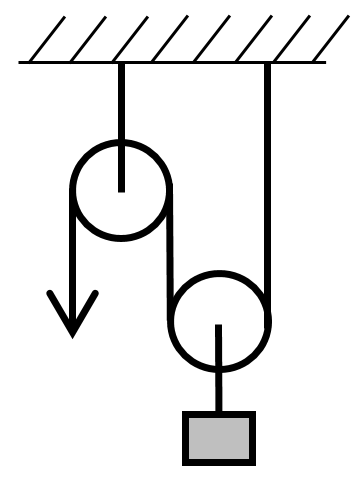
\includegraphics[width = \textwidth / 5]{P-1}
    \caption{}
    \labelf{P-1}
    \vspace{-1cm}
\end{wrapfigure}
\subsection*{Problem}

The system supposed to lift weights
consists of a stationary and a movable pulleys
as shown in \reff{P-1}.
The radii of a pulley and its axis are $R$ and $r$ correspondingly.
Assume that the hole in the pulley is slightly bigger than the axis.
There is a friction between the axis and the pulley
with a given friction coefficient $\mu$.
There is no sliding between the ropes and the pulleys,
as well as between the ropes and the axes.
Determine the energy efficiency coefficient of the system

\subsection*{Solution}

\begin{wrapfigure}{r}{.6\textwidth}
    \centering

    \begin{subfigure}[l]{.3\textwidth}
        \centering
        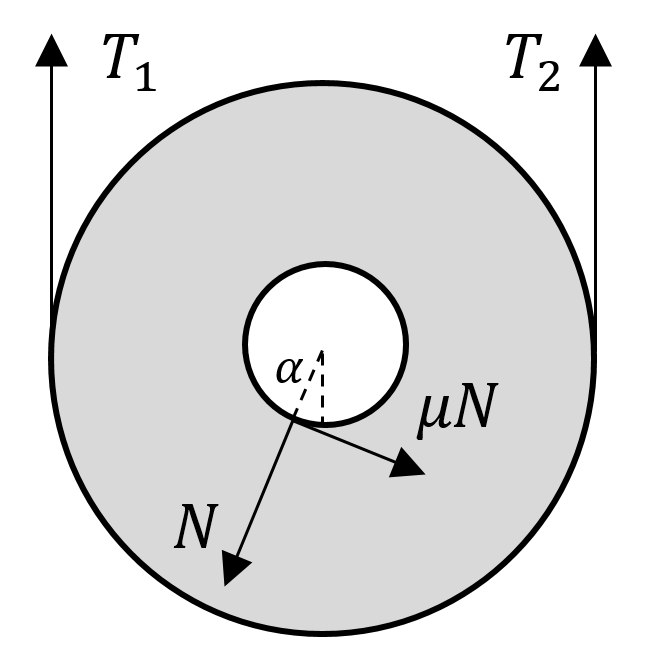
\includegraphics[width = \textwidth]{S-1}
        \caption{Forces on the pulley.}
        \labelf{S-1}
    \end{subfigure}
    \hfill
    \begin{subfigure}[l]{.29\textwidth}
        \centering
        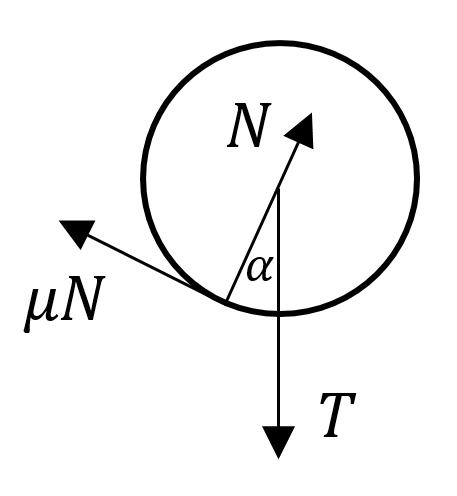
\includegraphics[width = \textwidth]{S-2}
        \caption{Forces on the axis.}
        \labelf{S-2}
    \end{subfigure}
    
    \caption{The forces on the movable pulley.}
    \labelf{S-1-2}
    \vspace{-1cm}
\end{wrapfigure}

Consider the movable pulley.
Let's assume, that in the process of lifting
the touching point between the pulley and its axis
is shifted left by some angle $\alpha$.
The forces acting on the pulley and the axis are shown in \reff{S-1-2}.
From the equilibrium on the axis we have
\begin{equation}
\begin{split}
    N \sin{\alpha} = \mu N \cos{\alpha} \\
    N \cos{\alpha} + \mu N \sin{\alpha} = T
\end{split}
\end{equation}
from where we get
\begin{equation}
\begin{split}
    \tan{\alpha} &= \mu \\
    \mu N = &T \frac{\mu}{\sqrt{1 + \mu^2}}
\end{split}
\end{equation}
Notice that we are not allowed to write toque equilibrium
as there is nothing known about the torque of interaction
between the axis and the rope attached to it.

The equilibrium of the pulley itself is written as
\begin{equation}
\begin{split}
    T_1 + T_2 = N \cos{\alpha} + \mu N \sin{\alpha} &\implies T_1 + T_2 = T \\
    R T_1 - R T_2 = r \mu N &\implies T_1 - T_2 = T \frac{r}{R} \frac{\mu}{\sqrt{1 + \mu^2}}
\end{split}
\end{equation}
and the other equation is identical to that of the axis.
From there we get
\begin{equation}
    T_{1/2} = T \frac{1 \pm \varepsilon}{2} , \hspace{1cm}
    \varepsilon = \frac{r}{R} \frac{\mu}{\sqrt{1 + \mu^2}}
\end{equation}

The situation and the equations for the stationary pulley
are absolutely the same as the ones written here.
So the tension of the free end of the rope should be
\begin{equation}
    T_0 = mg \cdot \frac{1+\varepsilon}{2} \cdot \frac{1+\varepsilon}{1-\varepsilon}
\end{equation}
so for the efficiency coefficient we get
\begin{equation}
    \eta = \frac{mg l}{T_0 \cdot 2l} = \frac{1 - \varepsilon}{(1 + \varepsilon)^2}
\end{equation}
